 \documentclass{beamer}
 
 \usepackage{amsmath}
 \usepackage{graphics}
 \usepackage{graphicx}
 \usepackage{framed}
 \usepackage{amssymb}
 
 \begin{document}
 	%==============================================================================================%
 	\begin{frame}
 		% % SLIDE 1 - COVER SLIDE
 		\begin{figure}
 			\centering
 			
\includegraphics[width=0.9\linewidth]{Rlogo}
 		\end{figure}
 		\[ \mbox{Introduction to R} \] 
 	\end{frame}
 	
 	%==============================================================================================%
 	\begin{frame}
 		\frametitle{Introduction to R}
 		Source: R project website (http://www.r-project.org)
 		\begin{itemize}
 			\item R is a language and environment for statistical computing and graphics. It is a GNU project
 			which is similar to the S language and environment which was developed at Bell Laboratories
 			(formerly AT\&T, now Lucent Technologies) by John Chambers and colleagues. 
 			\item R can be considered
 			as a different implementation of S. There are some important differences, but much
 			code written for S runs unaltered under R.
 		\end{itemize}
 		
 	\end{frame}
 	
 	%==============================================================================================%
 	\begin{frame}
 		\frametitle{What is R?}
 		\begin{itemize}
 			\item R provides a wide variety of statistical (linear and nonlinear modelling, classical statistical tests,
 			time-series analysis, classification, clustering, ...) and graphical techniques, and is highly extensible.
 			\item The S language is often the vehicle of choice for research in statistical methodology,
 			and \texttt{R} provides an Open Source route to participation in that activity.
 			\item One of \texttt{R}’s strengths is the ease with which well-designed publication-quality plots can be
 			produced, including mathematical symbols and formulae where needed. 
 			\end{itemize}
 			
 		\end{frame}
 		
 		%==============================================================================================%
 		\begin{frame}
 			\frametitle{What is R?}
 			\begin{itemize}
 			\item Great care has been
 			taken over the defaults for the minor design choices in graphics, but the user retains full control.
 			\item \texttt{R} is available as Free Software under the terms of the Free Software Foundation’s GNU General
 			Public License in source code form. It compiles and runs on a wide variety of UNIX platforms
 			and similar systems (including FreeBSD and Linux), Windows and MacOS.
 		\end{itemize}
 	\end{frame}
 	%==============================================================================================%
 	\begin{frame}
 		
 		\frametitle{What is R?}
 		\texttt{R} is a programming environment that
 		\begin{itemize}
 			\item uses a well-developed but simple programming language
 			\item allows for rapid development of new tools according to user demand
 			\item these tools are distributed as packages, which any user can download to customize the R
 			environment.
 		\end{itemize}
 	\end{frame}
 	%==============================================================================================%
 	\begin{frame}
 		% % SLIDE 1 - COVER SLIDE
 		\begin{figure}
 			\centering
 			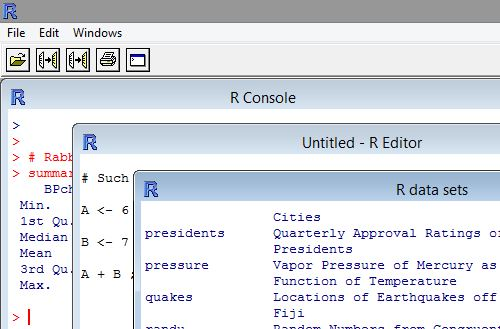
\includegraphics[width=1.2\linewidth]{images/Rmultiplewindows}
 		\end{figure}
 		
 	\end{frame}   
 	
 	%==============================================================================================%
 	\begin{frame}
 		\frametitle{Comprehensive R Archive Network}
 		\begin{itemize}
 			\item Base \texttt{R} and most \texttt{R} packages are available for download from the \textbf{Comprehensive R Archive Network}
 			(CRAN) cran.r-project.org. 
 			\item Base \texttt{R} comes with a number of basic data management,
 			analysis, and graphical tools 
 			\item \texttt{R}s power and flexibility, however, lie in its array of packages
 			(currently more than 6,000!)
 		\end{itemize}
 		
 	\end{frame}
%======================================================================================= % 	
  	\begin{frame}
 		\begin{figure}
\centering
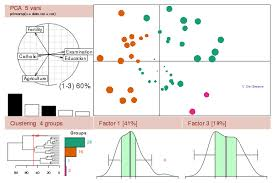
\includegraphics[width=1.2\linewidth]{CRAN}
\end{figure}
 	\end{frame}
 	%============================================================================= %
 	\begin{frame}
 		\frametitle{Introduction to R}
\textbf{Secton 1 - A few basics} 
		\begin{itemize}
 			\item[1.1] Installing \texttt{R}      
 			\item[1.2] Command Line Interface     
 			\item[1.3] The Assignment operator     
 			\item[1.4] Commenting      
 			\item[1.5] Defining Variables     
 			\item[1.6] Help Functions      
 			\item[1.7] The \texttt{help.start()} command     
 			\item[1.8] Basic Maths Operations     
 			\item[1.9] Basic \texttt{R} Editor      
 		\end{itemize}
 	\end{frame}
 	%==============================================================================================%
 	\begin{frame}
 		\frametitle{1.1 Installing R}
 		\begin{itemize}
 			\item \texttt{R} is very easily installed by downloading it from the CRAN website. Installation usually takes
 			about 2 minutes. 
 			\item When installation of R is complete, the distinctive \texttt{R} icon will appear on your
 			desktop. To start \texttt{R}, simply click this Icon. 
 			\item It is common to re-install \texttt{R} once a year or so. The
 			current version of \texttt{R}, version 3.1.2 was released quite recently.
 		\end{itemize}
 		
 	\end{frame}
 	
 	
 	%==============================================================================================%
 	\begin{frame}
 		% % SLIDE 1 - COVER SLIDE
 		\begin{figure}
 			\centering
 			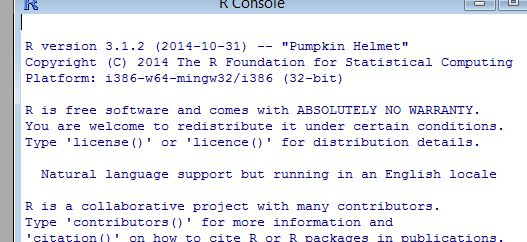
\includegraphics[width=1.2\linewidth]{images/Rversion}        
 		\end{figure}
 	\end{frame}  
 	%==============================================================================================%
 	\begin{frame}
 		
 		\frametitle{1.2 Command Line Interface}
 		\begin{itemize}
 			\item When you start \texttt{R}, the command line interface window will appear on screen. This is one
 			of many windows in the \texttt{R} environment, others including graphical output windows, or script
 			editors. 
 			\item \texttt{R} code can be entered into the command line directly. 
 			\item Alternatively code can be saved
 			to a script, which can be run inside a session using the \texttt{source()} function.
 		\end{itemize}
 	\end{frame}
 	%==============================================================================================%
 	\begin{frame}
 		\frametitle{1.3 The Assignment operator}
 		\begin{itemize}
 			\item The assignment operator is used to assign names to particular values. 
 			\item Historically the assignment
 			operator was ) a ``\texttt{$<-$}”. 
 			\item The assignment operator can also be the equals sign "=". (This is valid as of \texttt{R}
 			version 1.4.0.)
 			
 			\item Both will be used, although, you should learn one and stick with it. Many long term \texttt{R}
 			users prefer the arrow approach. 
 		\end{itemize}
 	\end{frame}
 	
 	%==============================================================================================%
 	\begin{frame}
 		\frametitle{1.3 The Assignment operator}
 		\begin{itemize}
 		\item You can also use $->$ as an assignment operator, reversing the
 		usual assignment positions. (This is actually really useful).
 		\item Commands are separated either by
 		a semi colon or by a newline.
 		\end{itemize}
 		\begin{figure}
 			\centering
 			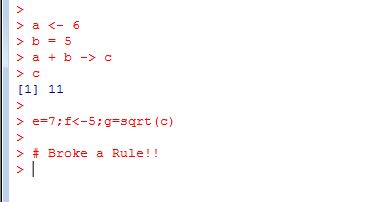
\includegraphics[width=1.2\linewidth]{images/assignment}
 			%\caption{}
 			%\label{fig:assignment}
 		\end{figure}
 		
 	\end{frame}
 	
 	%==============================================================================================%
 	\begin{frame}
 		\frametitle{1.3 The Assignment operator}
 		\textbf{The Up and Down Keys}
 		\begin{itemize}
 			\item Before we continue, try using the up and down keys, and see what happens. 
 			\item Previously
 			typed commands are re-presented, and can be re-executed.
 		\end{itemize}
 		
 	\end{frame}
 	%==============================================================================================%
 	\begin{frame}
 		\frametitle{1.3 The Assignment operator }
 		\textbf{objects}
 		\begin{itemize}
 			\item R stores both data and output from data analysis (as well as everything else) in \textbf{objects}.
 			\item The variables we have created so far are objects. 
 			\item A list of all objects in the current session can
 			be obtained with \texttt{ls()}.
 		\end{itemize}
 	\end{frame}
 	\textbf{1.3.1 Reserved Words - Bad names for Objects}
 	\begin{itemize}
 		\item Some names are used by the system, e.g.\texttt{T, F,q,c} etc . 
 		\item Avoid using these. (This is the rule I broke earlier on)
 		\item Also avoid using command names like \textbf{mean} and \textbf{sum}
 	\end{itemize}
 	
 	
  
 	%==============================================================================================%
 	\begin{frame}
 		\frametitle{1.4 Commenting}
 		For the sake of readability, it is good practice to comment code. The \# character at the
 		beginning of a line signifies a comment, which is not executed. Lines of hashtags can be used
 		to identify the beginning and end of code segments
 		\begin{figure}
 			\centering
 			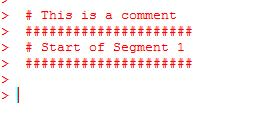
\includegraphics[width=1.2\linewidth]{images/commenting}
 			%\caption{}
 			%\label{fig:commenting}
 		\end{figure}
 		
 	\end{frame}
 	%==============================================================================================%
 	\begin{frame}
 		\frametitle{1.5 Defining and Naming Variables}
 		\begin{itemize}
 			\item A convention is to use define a variable name with a capital letter (R is case sensitive). 
 			\item This
 			reduces the chance of overwriting in-build \texttt{R} functions, which are usually written in lowercase
 			letters. 
 			\item Commonly used variable names such as x, y and z (in lower case letters) are not “reserved”.
 		\end{itemize}
 		\textbf{Camel Case}
 		\begin{framed}
 			\texttt{camelCase}
 			
 			\texttt{variableName}
 			
 			\texttt{AlsoCamelCase}
 		\end{framed}
 	\end{frame}

 	%==============================================================================================%
 	\begin{frame}
 		
 		\frametitle{1.6 Help Functions}
 		\begin{itemize}
 			\item  Help files for R functions are accessed by preceding the name of the function with ?\\  (e.g. \texttt{?sort}
 			). 
 			
 			\item Alternatively you can use the command \texttt{help()} (e.g. \texttt{help(sqrt)} )
 		\end{itemize}
 		
 	\end{frame}
 	%==============================================================================================%
 	\begin{frame}
 		
 		\frametitle{1.6 Help Functions}
 		\begin{itemize}
 			\item A HTML document appears on screen with information on the function typed in. 
 			\item As well
 			as the list of arguments that the particular function accepts, and how to specify them, there is
 			example code at the bottom of the file. 
 			\item These code segments are often invaluable in learning
 			how to master the function.
 		\end{itemize}
 		
 		
 	\end{frame}
 	
 	%==============================================================================================%
 	\begin{frame}
 		% % SLIDE 1 - COVER SLIDE
 		\begin{figure}
 			\centering
 			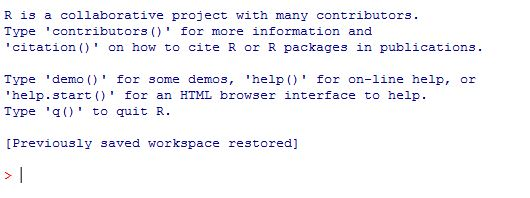
\includegraphics[width=1.2\linewidth]{images/Rhelpcommands}
 			%%\caption{}
 			%%\label{fig:Rhelpcommands}
 		\end{figure}
 	\end{frame}   
 	
 	
 
 	%==============================================================================================%
 	\begin{frame}
 		
 		
 		\frametitle{1.7 The \texttt{help.start()} command}
 		As mentioned by the text on the main console, the \texttt{help.start()} command can be usd to
 		access detailed help documentation that comes as part of the installation.
 	\end{frame}
 	
 	\begin{frame}\begin{figure}
\centering
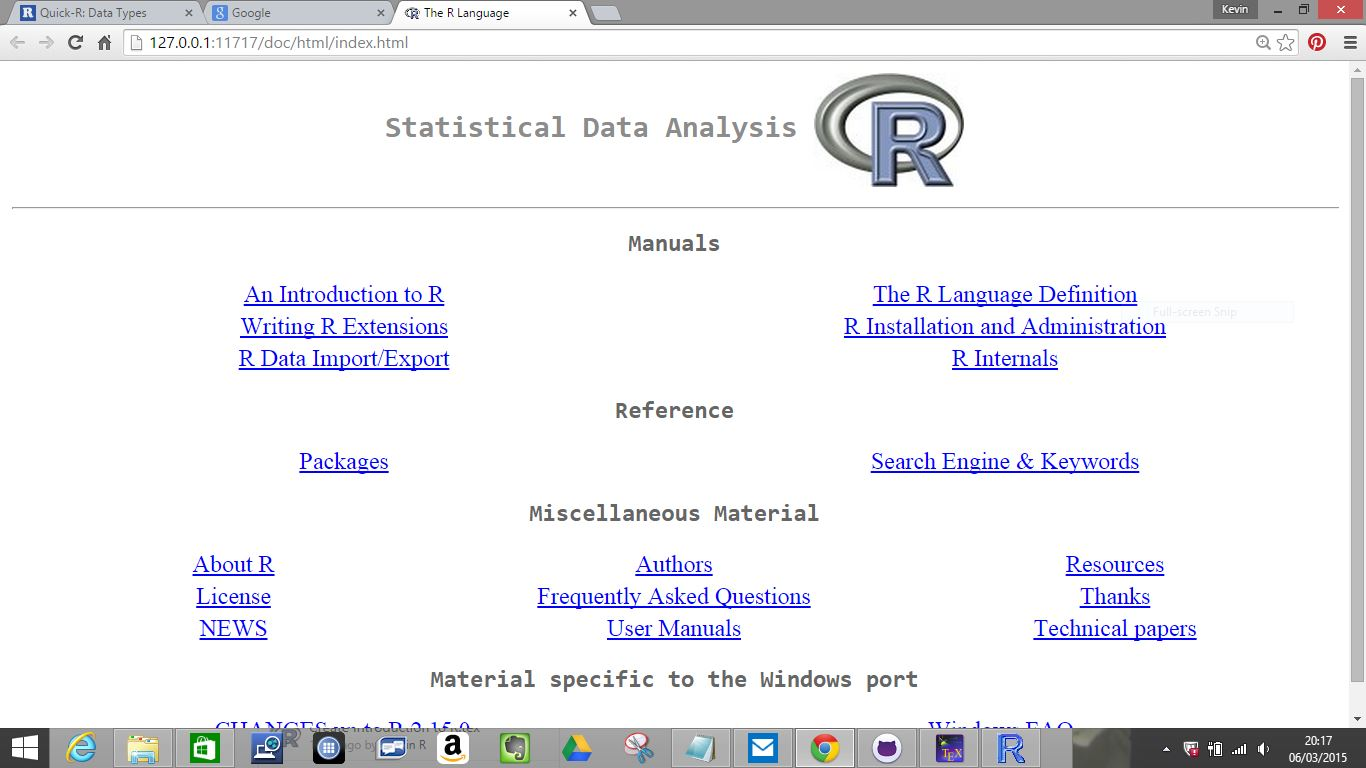
\includegraphics[width=1.2\linewidth]{images/helpstart}

\end{figure}
\end{frame}
 	%==============================================================================================%
 	\begin{frame}
 		
 		\frametitle{1.8 Basic Maths Operations}
 		\vspace{-0.5cm}
 		The most commonly used mathematical operators are all supported by \texttt{R}. \\ \bigskip Here are a few
 		examples:
 		\begin{tabular}{|c|c|} \hline
 			$5 + 3 \ast 5$ &  Note the order of operations.\\\hline
 			log (10) & Natural logarithm with base e=2.718282 \\\hline
 			log(8,2) & Log to the base 2 \\\hline
 			$4^2$ & 4 raised to the second power \\\hline
 			7/2 & Division \\\hline
 			factorial(4) & Factorial of Four \\\hline
 			sqrt (25) & Square root \\\hline
 			abs (3-7) & Absolute value of 3-7 \\\hline
 			pi & The mysterious number \\\hline
 			exp(2) & exponential function \\\hline
 			
 		\end{tabular} 
 	\end{frame}
 	
 	%==============================================================================================%
 	\begin{frame}
 		
 		\texttt{R} can be used for many mathematical operations, including
 		
 		\begin{itemize}
 			\item Set Theory
 			\item Trigonometry
 			\item Complex Numbers
 			\item Binomial Coefficients
 		\end{itemize}
 		Set Theory is always useful to know (Monty Hall Problem). We will not go into any of the others in great detail today.
 	\end{frame}

 	%==============================================================================================%
 	\begin{frame}
 		\frametitle{1.9 Basic \texttt{R} Editor}
 		\begin{itemize}
 		\item \texttt{R} has an inbuilt script editor. We will use it for this class, but there are plenty of top quality
 		Integrated Development Environments out there. (Read up about \textbf{RStudio} for example).
 		\item For a while, we will use the in-built script editor. Although it is advisable to start using \textbf{Rstudio} or something similar in the not-too-distant future.
 		\end{itemize}
 		
 	\end{frame}
 	
 		%==============================================================================================%
 		\begin{frame}
 			% % SLIDE 1 - COVER SLIDE
 			\begin{figure}
 				\centering
 				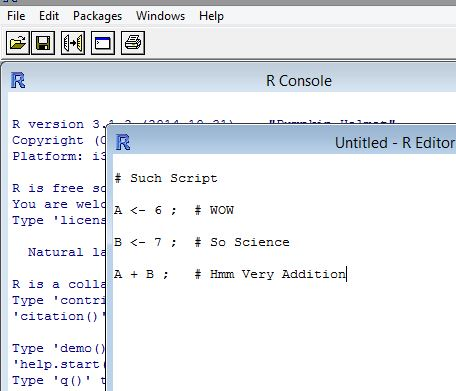
\includegraphics[width=1.2\linewidth]{images/Rscript}         
 			\end{figure}
 		\end{frame}   
 	%==============================================================================================%
 	\begin{frame}
 		\frametitle{1.9 Basic \texttt{R} Editor}
 		\begin{itemize}
 		\item To start a new script, or open an existing script simply go to File and click the appropriate
 		options. A new dialogue box will appear. 
 		
 		\item You can write and edit code using this editor.
 		\item To pass the code for compiling , press the run line or selection option (The third icon
 		on the menu).
 		\end{itemize}
 	\end{frame}
 	%==============================================================================================%
 	\begin{frame}
 		
 		\begin{itemize}
 		\item Another way to read code is to use the \texttt{edit()} function, which operates directly from the
 		command line. 
 		\item To see how the code defining an object X was written (or more importantly,
 		could have been written) simply type \texttt{edit(X)}. 
 		\item This command has some useful applications
 		that we will see later on (the \texttt{scan()} command).
 		\end{itemize}
 		
 	\end{frame}
 	%==============================================================================================%
 	\begin{frame}
 		
 		\textbf{Script Files}
 		\begin{itemize}
 			\item Scripts are saved as \texttt{.R} files. 
 			\item These scripts can be called directly using the \texttt{source()} command.
 		\end{itemize}
 		
 		\begin{framed}
 	\texttt{source(myScript.R)}
 		
 		\texttt{source(myDatasets.R)}
 		
 		\texttt{source(myFunctions.R)}
 	\end{framed}
 	\end{frame}
 	
 	%============================================================================= %
 	\begin{frame}
 		\frametitle{Introduction to R - Continued}
 		\begin{itemize}
 			\item[1.10] Built-In Data Sets      
 			\item[1.11] The \texttt{summary()} command     
 			\item[1.12] Working directories      
 			\item[1.13] Coming Unstuck    
 			\item[1.14] Quitting the \texttt{R} environment   
 			\item[1.15] Data Objects  
 			\item[1.16] Listing all items in a workspace     
 			\item[1.17] Removing items   
 			\item[1.18] Checking and Transforming Types
 			\item[1.19] Saving and Loading R Data Objects    
 		\end{itemize}
 	\end{frame}
 	
 	
 	%==============================================================================================%
 	\begin{frame}
 		\frametitle{1.10 Built-In Data Sets}
 		\textbf{Inbuilt Data Sets}\\
 		Several data sets , intended as learning tools, are automatically installed when R is installed.
 		Many more are installed within packages to complement learning to use those packages. \\
 		\bigskip
 		
 		\textbf{iris}\\ One
 		of these is the famous Iris data set, which is used in many data mining exercises.
 		
 		\begin{itemize}
 			\item airquality  ( very useful )
 			\item mtcars
 			\item Nile
 		\end{itemize}
 		More are available once packages are loaded.
 		
 	\end{frame}
 	%==============================================================================================%
 	\begin{frame}
 		% % SLIDE 1 - COVER SLIDE
 		\begin{figure}
 			\centering
 			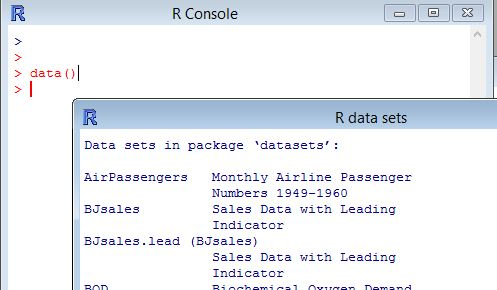
\includegraphics[width=1.2\linewidth]{images/Rdatasets}        
 		\end{figure}
 	\end{frame}   
 	%==============================================================================================%
 	\begin{frame}
 		% % SLIDE 1 - COVER SLIDE
 		\begin{figure}
 			\centering
 			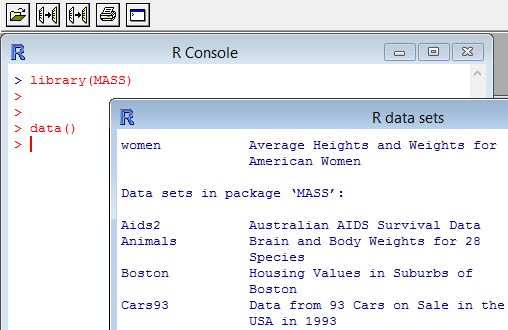
\includegraphics[width=1.2\linewidth]{images/RdatasetsMore}   
 		\end{figure}
 	\end{frame}   
 	%==============================================================================================%
 	\begin{frame}
 		
 		\begin{itemize}
 			\item To see what data sets are available, simply type \texttt{data()}.
 			\item  To load a data set, simply type in the
 			name of the data set. Some data sets are very large.
 			\item  To just see the first few (or last) rows, we
 			use the \texttt{head()} function or alternatively the \texttt{tail()} function. 
 			\item The default number of rows of
 			these commands is 6. Other numbers can be specified.
 		\end{itemize}
 		
 	\end{frame}
 	%==============================================================================================%
 	\begin{frame}
 		% % SLIDE 1 - COVER SLIDE
 		\begin{figure}
 			\centering 
 			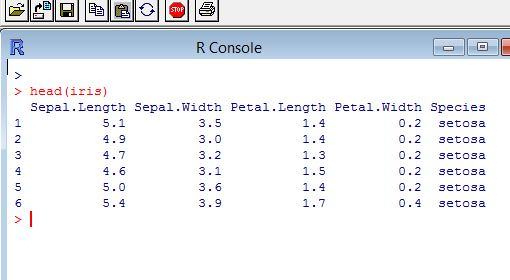
\includegraphics[width=1.2\linewidth]{images/irishead}      
 		\end{figure}
 	\end{frame}   
 	%==============================================================================================%
 	\begin{frame}
 		% % SLIDE 1 - COVER SLIDE
 		\begin{figure}
 			\centering
 			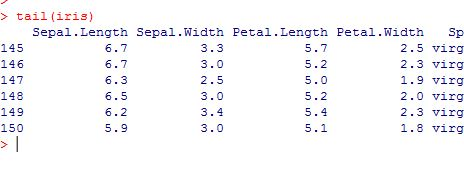
\includegraphics[width=1.2\linewidth]{images/iristail}     
 		\end{figure}
 	\end{frame}   
 	%==============================================================================================%
 	\begin{frame}
 		\begin{itemize}
 			\item In many situations, it is useful to call a particular data set using the \texttt{attach()} command. This
 			will save having to specify the data sets over repeated operations. 
 			\item The file can then be detached
 			using the \texttt{detach()} command.
 		\end{itemize}
 		
 		
 		
 	\end{frame}
 	%==============================================================================================%
 	\begin{frame}
 		\frametitle{1.11 The summary() command}
 		
 		\begin{itemize}
 		\item The R command \texttt{summary()} is a generic function used to produce result “summaries” of the
 		results of various objects, from simple vectors to the output of complex model fitting functions.
 		\item The function invokes particular methods which depend on the class of the first argument.
 		\end{itemize}
 	\end{frame}
 	%==============================================================================================%
 	\begin{frame}
 		% % SLIDE 1 - COVER SLIDE
 		\begin{figure}
 			\centering
 			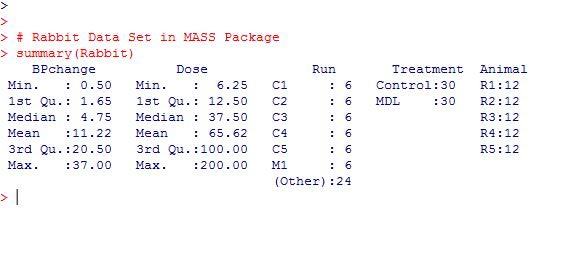
\includegraphics[width=1.2\linewidth]{images/rabbitsummary}   
 		\end{figure}
 	\end{frame} 
 	
 	%==============================================================================================%
 	\begin{frame}
 		% % SLIDE 1 - COVER SLIDE
 		\begin{figure}  
 			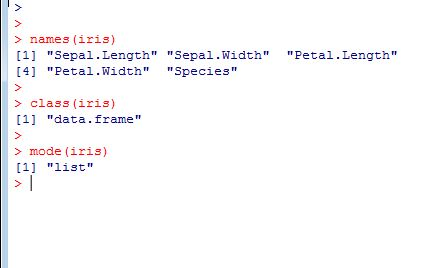
\includegraphics[width=1.2\linewidth]{images/irisinspect}     
 		\end{figure}
 	\end{frame}   
 	%==============================================================================================%
 	\begin{frame}
 		% % SLIDE 1 - COVER SLIDE
 		\begin{figure}
 			\centering
 			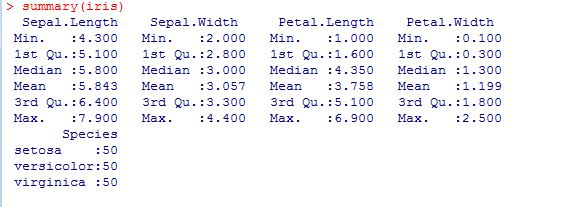
\includegraphics[width=1.2\linewidth]{images/irissummary}
 			%\caption{}
 			%\label{fig:irissummary}
 		\end{figure}
 	\end{frame}   
 	
 	
 	
 	
 	%==============================================================================================%
 	\begin{frame}
 		\frametitle{1.12 Working directories}
 		\large
 		\begin{itemize}
 			\item You can change your working directly by using the appropriate options on the File menu. 
 			\item To
 			determine the current working directory, you can use the \texttt{getwd()} command. 
 			\item To change the
 			working directory , we would use the \texttt{setwd()} command.
 			\item  This is quite important as objects
 			will be imported and exported to and from the specified directory.
 		\end{itemize}
 	\end{frame}
 	%==============================================================================================%
 	\begin{frame}
 		\begin{figure}
 			\centering
 			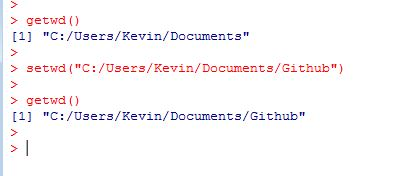
\includegraphics[width=1.2\linewidth]{images/workingdir}
 			
 		\end{figure}
 		
 	\end{frame}
 	

 	%==============================================================================================%
 	\begin{frame}
 		\frametitle{1.13 Coming Unstuck}
 		\Large
 		\begin{itemize}
 			\item  If you are having trouble with a piece of code that is currently compiling , all you have to do is press ESC, just like many other computing environments.
 		\end{itemize}  
 	\end{frame}
 	%==============================================================================================%
 	\begin{frame}
 		\frametitle{1.14 Quitting the R environment}
 		As the front page text indicates, all you have to do to quite the workspace is to type in \texttt{q()}.
 		You will then be prompted to save your work.
 	\end{frame}
 	%==============================================================================================%
 	\begin{frame}
 		\frametitle{1.15 Data Objects}
 		As mentioned previously, R saves data as \textbf{objects}. Examples of data objects are
 		\begin{itemize}
 			\item Vectors
 			\item Lists
 			\item Dataframes
 			\item Matrices
 		\end{itemize}
 		The simple objects we have created previously are simply single element vectors.
 	\end{frame}
 	%==============================================================================================%
 	\begin{frame}
 		\frametitle{1.16 Listing all items in a workspace}
 		To list all items in an R environment, we use the \texttt{ls()} function. This provides a list of all data
 		objects accessible. Another useful command is \texttt{objects()}.
 		\begin{figure}
 			\centering
 			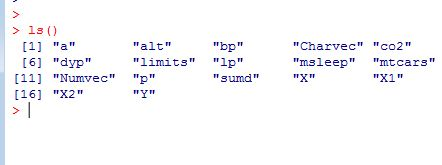
\includegraphics[width=1.2\linewidth]{images/ObjectsList}
 			%\caption{}
 			%\label{fig:ObjectsList}
 		\end{figure}
 		
 	\end{frame}
 	%==============================================================================================%
 	\begin{frame}
 		\frametitle{1.17 Removing items}
 		\begin{itemize}
 			\item Sometimes it is desirable to save a subset of your workspace instead of the entire workspace.
 			\item One option is to use the \texttt{rm()} function to remove unwanted objects right before exiting your R
 			session; another possibility is to use the \texttt{save()} function.
 		\end{itemize}
 	\end{frame}
 	
 	
 
 	%==============================================================================================%
 	\begin{frame}
 		\frametitle{1.19 Saving and Loading R Data Objects}
 		In situations where a good deal of processing must be used on a raw dataset in order to prepare
 		it for analysis, it may be prudent to save the R objects you create in their internal binary form.
 		One attractive feature of this scheme is that the objects created can be read by R programs
 		running on different computer architectures than the one on which they were created, making it
 		very easy to move your data between different computers. Each time an R session is completed,
 		you are prompted to save the workspace image, which is a binary file called .RData in the
 		working directory.
 	\end{frame}
 	%==============================================================================================%
 	\begin{frame}
 		Whenever R encounters such a file in the working directory at the beginning of a session,
 		it automatically loads it making all your saved objects available again. So one method for
 		
 		saving your work is to always save your workspace image at the end of an R session. If you
 		would like to save your workspace image at some other time during your R session, you can use
 		the save.image() function, which, when called with no arguments, will also save the current
 		workspace to a file called .RData in the working directory.
 		
 	\end{frame}
 	%============================================================================= %
 	\begin{frame}
 		\frametitle{Introduction to R (Continued) }
 		\begin{itemize}
 			\item[2.1] Three particularly useful commands    
 			\item[2.2] Changing GUI options     
 			\item[2.3] Colours      
 			\item[2.4] Use of the Semi-Colon Operator     
 			\item[2.5] The \texttt{apropos()} Function     
 			\item[2.6] History       
 			\item[2.7] The \texttt{sessionInfo()} Function     
 			\item[2.8] Time and date functions     
 			\item[2.9] Logical States      
 			\item[2.10] Missing Data      
 			\item[2.11] Files in the Working Directory     
 		\end{itemize}
 	\end{frame}
 	
 	%==============================================================================================%
 	\begin{frame}
 		%    2 Introduction to R (Continued)
 		\frametitle{2.1 Some particularly useful commands}
 		
 		
 		The Holy Trinity
 		\begin{itemize}
 			\item \texttt{help()}
 			\item \texttt{summary()}
 			\item \texttt{help.start()}
 			\item \texttt{apropos()}
 		\end{itemize}
 		
 	\end{frame}
 	%==============================================================================================%
 	\begin{frame}
 		\frametitle{2.2 Changing GUI options}
 		\begin{itemize}
 			\item We can change the GUI options using the GUI preferences option on the Edit menu.
 			\item  (Important
 			when teaching R) 
 			\item A demonstration will be done in class.
 		\end{itemize}
 		
 	\end{frame}
 	%==============================================================================================%
 	\begin{frame}
 		\frametitle{2.3 Colours}
 		\begin{itemize}
 			\item R supported a massive number of colours.
 			\item Type in colours() (or colors()) to see what colours
 			are supported.
 		\end{itemize}
 	\end{frame}
 	
 	\begin{frame}
 		\begin{figure}
 			\centering
 			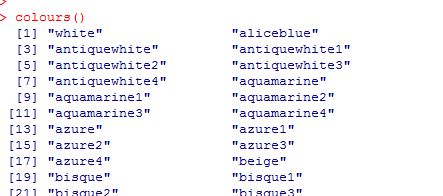
\includegraphics[width=1.2\linewidth]{images/Rcolours}
 			%\caption{}
 			%\label{fig:Rcolours}
 		\end{figure}
 		
 	\end{frame}
 	
 	 	%==============================================================================================%
 	\begin{frame}
 		\frametitle{2.4 Use of the Semi-Colon Operator}
 		\begin{itemize}
 			\item The semi-colon operator at the end of each line of code is not necessary in general, but using it
 			overcomes errors due to copying and pasting from document soft copies. 
 			\item It is also useful for compacting multiple short statements onto a single line.
 			\item In other programming
 			languages, such as Octave, using the semicolon in this way has a distinct purpose.
 		\end{itemize}
 	\end{frame}
 	%==============================================================================================%
 	\begin{frame}
 		\frametitle{2.5 The \texttt{apropos()} Function}
 		\begin{itemize}
 		\item This function is very useful for determining what functions are available for a particular topic,
 		although the process requires a great deal of trial and error. 
 		\item Suppose we are looking for a
 		command to print out the session information. 
 		\item We would use a very short string (e.g. \textbf{essio})
 		that would plausibly be part of useful function names.
 		\end{itemize}
 	\end{frame}
 	
 		%==============================================================================================%
 		\begin{frame}
 			% % SLIDE 1 - COVER SLIDE
 			\begin{figure}
 				\centering
 				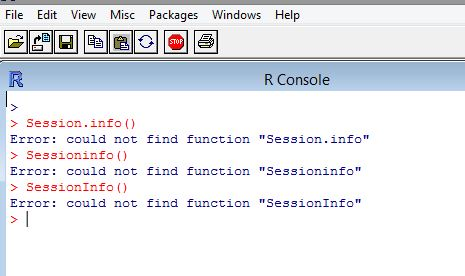
\includegraphics[width=1.2\linewidth]{images/Rapropos1}       
 			\end{figure}
 		\end{frame}   
 		%==============================================================================================%
 		\begin{frame}
 			% % SLIDE 1 - COVER SLIDE
 			\begin{figure}
 				\centering
 				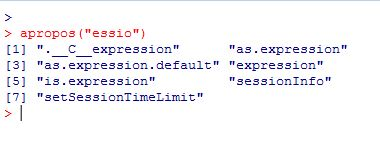
\includegraphics[width=1.2\linewidth]{images/Rapropos2}       
 			\end{figure}
 		\end{frame}   
 	%==============================================================================================%
 	\begin{frame}
 		\frametitle{2.6 History}
 		\begin{itemize}
 			\item The command \texttt{history()} is used to obtain the last 25 commands used by \texttt{R}.
 			\item 25 is the default number, you can specify another number.
 		\end{itemize}
 		
 		
 	\end{frame}
 	%==============================================================================================%
 	\begin{frame}
 		% % SLIDE 1 - COVER SLIDE
 		\begin{figure}
 			\centering
 			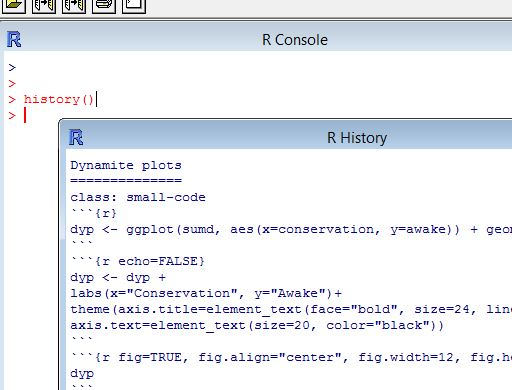
\includegraphics[width=1.2\linewidth]{images/Rhistory}        
 		\end{figure}
 	\end{frame}   
 	%==============================================================================================%
 	\begin{frame}
 		\frametitle{2.7 The \texttt{sessionInfo()} Function}
 		To get a description of the version of R and its attached packages used in the current session,
 		we can use the \texttt{sessionInfo()} function
 		
 	\end{frame}
 	
 	\begin{frame}
 		
 		\frametitle{2.7 The \texttt{sessionInfo()} Function}
 		\begin{figure}
 			\centering
 			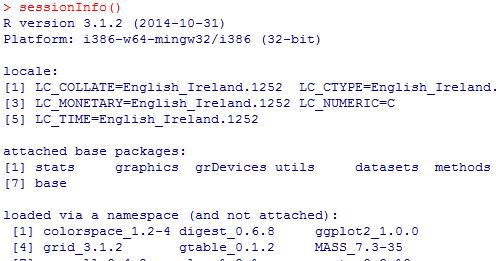
\includegraphics[width=0.99\linewidth]{images/sessionInfo}
 			%\caption{}
 			%\label{fig:sessionInfo}
 		\end{figure}
 	\end{frame}	
 	%==============================================================================================%
 	\begin{frame}
 		\frametitle{2.8 Time and date functions}
 		\begin{itemize}
 		\item The commands \texttt{Sys.time()} and \texttt{Sys.Date()} returns the system’s idea of the current date
 		with and without time. 
 		\item We can perform some simple algebraic calculations to compute time
 		differences (i.e. to find out how long some code took to compile).
 		\end{itemize}
 		
 	\end{frame}
 	%==============================================================================================%
 	\begin{frame}
 		\frametitle{System Time}
 		\begin{figure}
 			\centering
 			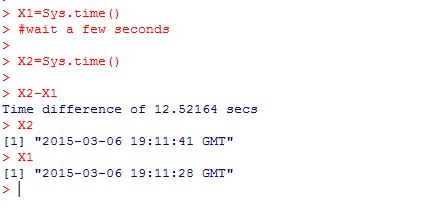
\includegraphics[width=1.2\linewidth]{images/Systime}
 			%\caption{}
 			%\label{fig:Systime}
 		\end{figure}
 		
 	\end{frame}
 	%==============================================================================================%
 	\begin{frame} 
 		\frametitle{2.9 Logical States}
 		\begin{itemize}
 			\item Logical states TRUE and FALSE are simply specified as such, all in capital letters. 
 			\item The
 			shortcuts T and F are also recognized
 		\end{itemize}
 	\end{frame}
 	%==============================================================================================%
 	\begin{frame}
 		\frametitle{2.10 Missing Data}
 		\begin{itemize}
 			\item In some cases the entire contents of a vector may not be known. For example, missing data
 			from a particular data set. \item A place can be reserved for this by assigning it the special value
 			NA.
 			NA is a logical constant of length 1 which contains a missing value indicator.
 			\item  NA stands
 			for Not Available.
 			\item Missing values can adversely affect calculations. Add \texttt{na.rm=T} to commands
 			
 			\begin{framed}
 			\texttt{mean(X,na.rm=T)}
 			\end{framed}
 		\end{itemize}
 	\end{frame}
 	%==============================================================================================%
 	\begin{frame}
 		
 		\frametitle{2.11 Files in the Working Directory}
 		It is possibel to call an R script from the working directory, using the \texttt{source()} function.
 		\begin{framed}
 			
 			\texttt{source("myfunctions.r")\\
 				source("mydata.r")}
 			
 		\end{framed} 
 		We can also send code put directly to a file in the working directory, using the \texttt{sink()}
 		command. The first time the command is used, the name of the created file is specified.
 		Subsequent commands print output directly to this file, until the command is used again to
 		cease the operation.
 	\end{frame}
 	%==============================================================================================%
 	\begin{frame}
 		\begin{figure}
 			\centering
 			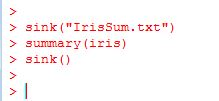
\includegraphics[width=1.2\linewidth]{images/sinkiris}
 			%\caption{}
 			%\label{fig:sinkiris}
 		\end{figure}
 		
 	\end{frame}

 	%==============================================================================================%
 	
 	\begin{frame}
 		\Huge
 		\[\mbox{ Section 3 : Inspecting a Data Set } \]
 	\end{frame}
 	%============================================================================= %
 	\begin{frame}
 		\frametitle{Section 3 - Inspecting a Data Set }
 		\begin{itemize}
 			\item[3.1] Dimensions of a data set 
 			\item[3.2] The \texttt{summary()} command   
 			\item[3.3] Structure of a Data Object 
 		\end{itemize}
 	\end{frame}
 	% %============================================================================= %
 	%\begin{frame}
 	%\frametitle{Section 4 : Packages}
 	%
 	%  \begin{semiverbatim}
 	%  4.1 Packages 
 	%  4.2 Using and Installing packages 
 	%  4.2.1 Version of R 
 	%  \end{semiverbatim}
 	%
 	% \end{frame}
 	%
 	%\end{document}
 	%============================================================================= %
 	% 	\begin{frame}
 	% 		\frametitle{Part 5 - Data Creation, Data Entry, Data Import and Export}
 	% 		\begin{framed}
 	% 			\begin{semiverbatim}
 	% 				5.1 The c() command 
 	% 				5.1.1 Vector of Numeric Values
 	% 				5.1.2 Vector of Character Values
 	% 				5.1.3 Vector of Logical Values 
 	% 				5.2 The scan() command 
 	% 				5.2.1 Characters with the scan() command
 	% 				5.3 Using the data editor
 	% 				5.4 Spreadsheet Interface 
 	% 			\end{semiverbatim}
 	% 		\end{framed}
 	% 		
 	% 	\end{frame}
 	
 	%==============================================================================================%
 	\begin{frame}
 		\frametitle{Section 3 Inspecting a Data Set}
 		\large 
 		\textbf{Summary of useful commands}
 		\begin{itemize}
 			\item \texttt{dim()} and \texttt{length()}
 			\item \texttt{nrow()} and \texttt{ncol()}
 			\item \texttt{names()}
 			\item \texttt{summary()}
 			\item \texttt{tail()}
 			\item \texttt{head()}
 			\item \texttt{describe()} (from the \textbf{psych} package)
 		\end{itemize}
 	\end{frame}
 	%==============================================================================================%
 	\begin{frame}
 		
 		\frametitle{3.1 Dimensions of a data set}
 		\begin{itemize}
 			\item We have remarked that some data sets are very large. 
 			\item This is perhaps a good place to consider
 			summary information about data objects. 
 			\item For a simple vector, a useful command to determine
 			the length (remark: sample size) is the function \texttt{length()}.
 		\end{itemize}
 		\begin{framed}
 			\texttt{Y=4:18}
 			\texttt{length(Y)}
 			
 		\end{framed}
 		For more complex data sets ( and data frames which we will see later) , we have several
 		tools for assessing the size of data.
 	\end{frame}
 	%==============================================================================================%
 	\begin{frame}
 		\begin{figure}
 			\centering
 			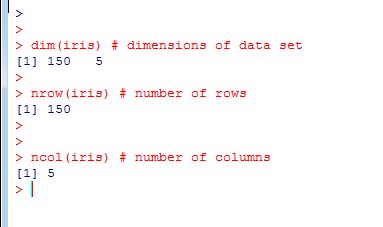
\includegraphics[width=1.2\linewidth]{images/dimsiris}
 			%\caption{}
 			%\label{fig:dimsiris}
 		\end{figure}
 		
 		
 		
 	\end{frame}
 	%==============================================================================================%
 	\begin{frame}
 		\frametitle{Column (Variable) names and Row names}
 		\begin{itemize}
 			\item We can also determine the row names and column names using the functions \texttt{rownames()}
 			and \texttt{colnames()}. 
 			\item If there are no specific row or column names, the command will just return
 			the indices.
 		\end{itemize}
 		\begin{figure}
 			\centering
 			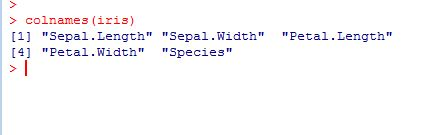
\includegraphics[width=1.0\linewidth]{images/colnamesiris}
 			%\caption{}
 			%\label{fig:colnamesiris}
 		\end{figure}
 		
 	\end{frame}
 	%==============================================================================================%
 	\begin{frame}
 		\frametitle{3.2 The \texttt{summary()} command}
 		\begin{itemize}
 			\item The command \texttt{summary()} is one of the most useful commands in \texttt{R}. 
 			\item It is a generic function used
 			to produce result summaries of the results of various functions. 
 			\item The function invokes particular
 			methods which depend on the class of the first argument. 
 			\item In other words, \texttt{R} picks out the most
 			suitable type of summary for that data.
 		\end{itemize}
 	\end{frame}
 	%==============================================================================================%
 	\begin{frame}
 		
 		
 		\begin{figure}
 			\centering
 			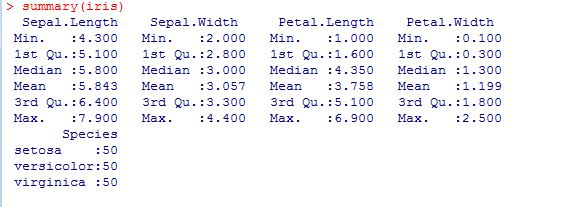
\includegraphics[width=0.99\linewidth]{images/irissummary}
 			
 		\end{figure}
 		\texttt{summary()} is particularly useful for manipulating data from more complex data objects.
 		
 	\end{frame}
 	%==============================================================================================%
 	\begin{frame}
 		
 		\frametitle{3.3 Structure of a Data Object}
 		\large
 		The structure, class and storage mode of an object can be determined using the following
 		commands. Try out a few.
 		\begin{itemize}
 			\item  \texttt{str()}
 			\item  \texttt{class()}
 			\item  \texttt{mode()}
 		\end{itemize}
 		
 		
 	\end{frame}
 	%==============================================================================================%
 	\begin{frame}
 		\begin{figure}
 			\centering
 			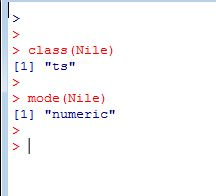
\includegraphics[width=0.7\linewidth]{images/classnile}
 			%\caption{}
 			%\label{fig:classnile}
 		\end{figure}
 		
 		
 	\end{frame}
 	%==============================================================================================%
 	\begin{frame}
 		\begin{figure}
 			\centering
 			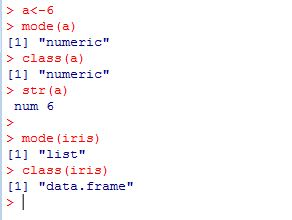
\includegraphics[width=0.9\linewidth]{images/modeclass}
 			
 		\end{figure}
 		
 		
 	\end{frame}
 	
 		%==============================================================================================%
 		\begin{frame}
 			\frametitle{Checking and Transforming Types}	
 			
 			\begin{itemize}
 			\item The \texttt{is} family of commands can check if an object is of a certain type.

\item The \texttt{as} family of commands can (often) convert an object to a specified type (in some cases not feasible). 			
\end{itemize}
 		\end{frame}
 		
 		
 		%==============================================================================================%
 		\begin{frame}
 				\frametitle{Checking and Transforming Types}	
 			% % SLIDE 1 - COVER SLIDE
 			\begin{figure}
 				\centering
 				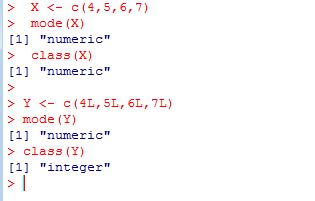
\includegraphics[width=1.2\linewidth]{images/numerictypes}    
 			\end{figure}
 		\end{frame} 
 		%==============================================================================================%
 		\begin{frame}
 			
 				\frametitle{Checking and Transforming Types}	
 			% % SLIDE 1 - COVER SLIDE
 			\begin{figure}
 				\centering
 				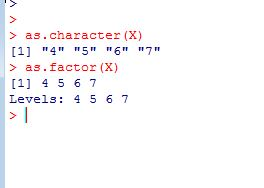
\includegraphics[width=1.2\linewidth]{images/typeconversion} 
 			\end{figure}
 		\end{frame}   
 	%==============================================================================================%
 	
 	\begin{frame}
 		\Huge
 		\[\mbox{ Section 4 : Packages } \]
 	\end{frame}
 	\begin{frame}
 		\frametitle{Packages}
 		
 		\begin{itemize}
 			\item A Package in \texttt{R} is a file containing a collection of objects which have some common purpose.
 			\item Packages enhance the capabilties and scope for research in a certain field. 
 			\item For example, the
 			package MASS contains objects associated with the Venables and Ripleys ``\textit{Modern Applied
 				Statistics with S}”. 
 		\end{itemize}
 		
 	\end{frame}
 	%=================================================================== %
 	\begin{frame}
 		
 		
 		\begin{figure}
 			\centering
 			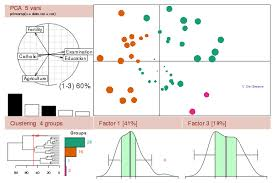
\includegraphics[width=0.97\linewidth]{CRAN}
 			%\caption{Comprehensive R Archive Network}
 			
 		\end{figure}
 		
 		
 	\end{frame}
 	
 	
 	%=================================================================== %
 	\begin{frame} 
 		\frametitle{R Packages}
 		
 		\begin{itemize}
 			\item ``10 R packages I wish I knew about earlier" - Drew Conway (Yhat.com, February 2013)
 			\bigskip \item ``The HadleyVerse" - Hadley Wickham
 			\begin{itemize}
 				
 				\item  ggplot2, dplyr, reshape, lubridate, stringr
 				
 				\item  With Romain Francois, Dianne Cook and Garret Grolemund.
 			\end{itemize}
 			\bigskip
 			\item Dr Brendan Haplin (UL): lme4 ,TraMineR, Gelman's arm, MASS, foreign. 
 			\bigskip
 			\item Shiny - Web Applications with \texttt{R}
 		\end{itemize}
 	\end{frame}
 	%=================================================================== %
 	\begin{frame} 
 		\frametitle{R Packages}
 		
 		\begin{itemize}
 		\item  	
 		Some examples of packages are Actuar, written for actuarial science, and
 		QRMlib, which complements the Quantitative Risk Management The command library()
 		lists all the available packages. 
 		
 		\item To load a particular package, for example MASS, we would
 		write
 	\end{itemize}\begin{framed}
 		\texttt{library(MASS)}
 		\end{framed}
 	\end{frame}
 	%=================================================================== %
 	\begin{frame}
 		
 		\frametitle{Packages}
 		\begin{itemize}
 			\item The CRAN package repository features 6107 available packages. 
 			\item Packages contain
 			various functions and data sets for numerous purposes, e.g.
 			\textbf{\textit{ggplot2}} package, \textbf{\textit{AER}} package, \textbf{\textit{survival}} package, etc.
 			\item Some packages are part of the basic installation. Others can be
 			downloaded from CRAN.
 			\item To access all of the functions and data sets in a particular package,
 			it must be loaded into the workspace. 
 			\item For example, to load the
 			\textbf{\textit{ggplot2}} package:
 		\end{itemize}
 		
 		\begin{framed}
 		\texttt{install.packages(ggplot2)}
 		
 		\texttt{library(ggplot2)}
 		\end{framed}
 	\end{frame}
 	%==============================================================================================%
 	\begin{frame}
 		\frametitle{4.2 Using and Installing packages}
 		\begin{itemize}
 			\item Many packages come with R. To use them in an R session, you need to load the package, as
 			previously demonstrated.
 			\item Some packages are not automatically installed when you install R but they need to be downloaded
 			and installed individually. 
 			\item We must first install them using the install.packages()
 			function, which typically downloads the package from CRAN and installs it for use. (follow the
 			instructions as indicated).
 		\end{itemize}
 	\end{frame}

 	%==============================================================================================%
 	\begin{frame}
 		\frametitle{4.2.1 Version of R}
 		Many packages will require you to have the most recent version of R and also other packages.
 		It is a good idea to update regularly.
 	\end{frame}
 	%==============================================================================================%
 	\begin{frame}
 		\[\mbox{Section 5 : Data Creation, Data Entry, Data Import and Export}\]
 	\end{frame}
 	%==============================================================================================%
 	\begin{frame}
 		\frametitle{5.1 The \texttt{c()} command}
 		To create a simple data set, known as a vector, we use the c() command to create the vector.
 		\begin{figure}
 			\centering
 			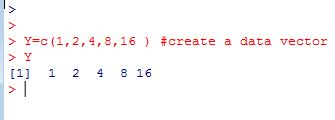
\includegraphics[width=1.2\linewidth]{images/makevector1}
 			%\caption{}
 			%\label{fig:makevector1}
 		\end{figure}
 		
 		
 	\end{frame}
 	%==============================================================================================%
 	\begin{frame}
 		\frametitle{Vectors}
 		\begin{figure}
 			\centering
 			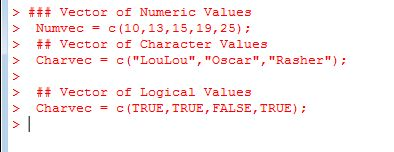
\includegraphics[width=1.2\linewidth]{images/makevectors}
 			%\caption{}
 			%\label{fig:makevectors}
 		\end{figure}
 		
 	\end{frame}
 	%==============================================================================================%
 	\begin{frame}
 		\frametitle{Vectors} 
 		Vectors can be bound together either by row or by column.
 		\begin{figure}
 			\centering
 			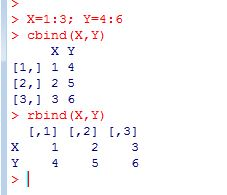
\includegraphics[width=1.0\linewidth]{images/cbindrbind}
 		\end{figure}
 		
 	\end{frame}
 	%==============================================================================================%
 	\begin{frame}
 		\frametitle{5.2 The scan() command}
 		\begin{itemize}
 			\item The \texttt{scan()} function is a useful method of inputting data quickly. 
 			\item You can use to quickly copy
 			and paste values into the \texttt{R} environment. It is best used in the manner as described in the
 			following example. 
 			\item Create a variable ”X” and use the \texttt{scan()} function to populate it with
 			values. 
 			\item Type in a value, and then press return. Once you have entered all the values, press
 			return again to return to normal operation.
 		\end{itemize}
 	\end{frame}
 	%==============================================================================================%
 	\begin{frame}
 		\begin{figure}
 			\centering
 			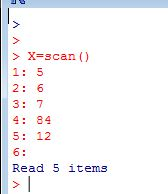
\includegraphics[width=0.8\linewidth]{images/scannumbers}
 			%\caption{}
 			%\label{fig:scannumbers}
 		\end{figure}
 		
 		Remark: Try the \texttt{edit()} command on object X.
 	\end{frame}
 	%==============================================================================================%
 	\begin{frame}
 		\frametitle{5.2.1 Characters with the scan() command}
 		The scan() command can also be used forinputting character data.
 		\begin{figure}
 			\centering
 			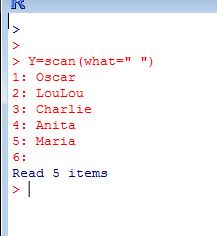
\includegraphics[width=0.7\linewidth]{images/scandognames}
 			%\caption{}
 			%\label{fig:scandognames}
 		\end{figure}
 		
 	\end{frame}
 	%==============================================================================================%
 	\begin{frame}
 		5.3 Using the data editor
 		
 	\end{frame}
 	%==============================================================================================%
 	\begin{frame}
 		\frametitle{5.4 Spreadsheet Interface}
 		\texttt{R} provides a spreadsheet interface for editing the values of existing data sets. We use the
 		command \texttt{data.entry()}, and name of the data object as the argument. (Also try out the
 		fix() command)
 		% 	\begin{framed}
 		% 		\begin{semiverbatim}
 		% 			> data.entry(X) # Edit the data set and exit interface
 		% 			> X
 		% 		\end{semiverbatim}
 		% 	\end{framed}
 		
 	\end{frame}
 	
 	
 	
 	
 	
 \end{document}